Note: I was playing around on my own Arduino Mega, forgot and took 
screenshots on it instead of the Uno. The code should still compile
fine for the Uno, I did not use anything extreme. I hope it isn't an 
issue, I'd disconnected everything by the time I realised.

\question*{
    Background and buildup: \texttt{analogWrite()} function
}

\begin{arabicparts}
    \questionpart
    \textbf{{Pins 3, 5, 6, 9, 10, and 11}.} Marked by $\sim$ on the board itself,
    confirmed with the Arduino documentation.\\
    The \texttt{analogWrite} system can be checked using an LED connected
    to it, followed by a large resistor, to ensure staying within current limits.

    \questionpart
    \textbf{0-255.} The value is limited by being an 8-bit unsigned interger type. A simple
    change in data type cannot mitigate this, since the counter on the Arduino itself
    is 8-bit only. There is supposedly another 16-bit counter per the ATmega328P datasheet,
    so not sure if that could be used to expand this further. However, in any case, the minute
    changes achievable by this method for the duty cycle might be bottlenecked by other
    hardware even \emph{if} they were of any practical purpose.

    \questionpart
    Connected circuit is as in Figure \ref{fig:pwmconnected}.
    \begin{figure}[ht]
        \centering
        \begin{subfigure}[b]{0.3\textwidth}
            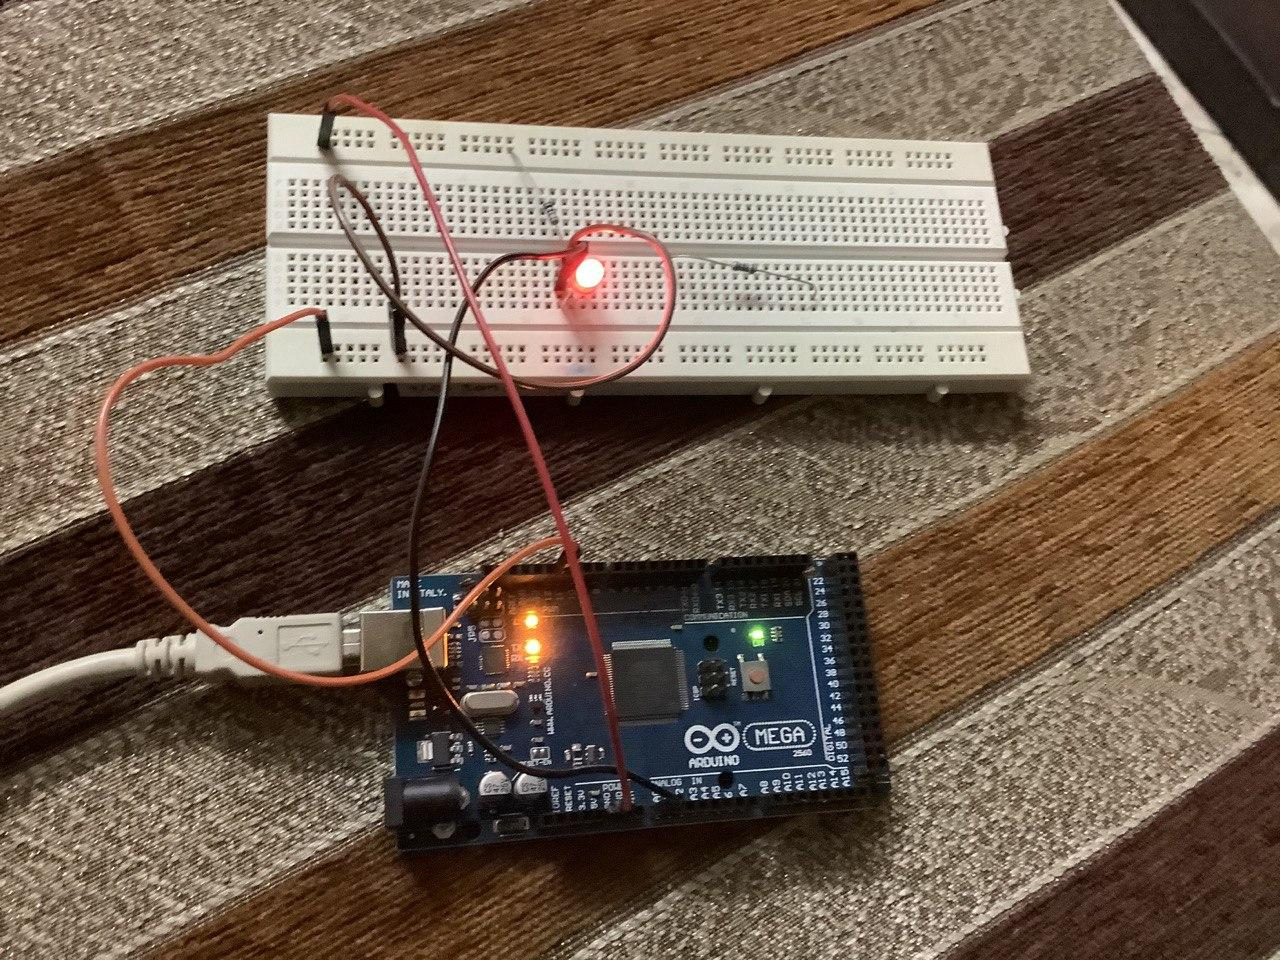
\includegraphics[width=\textwidth]{fig/pwm-low.jpg}
            \caption{Input \texttt{255/HIGH}}
            \label{subfig:pwmhigh}            
        \end{subfigure}
        \begin{subfigure}[b]{0.3\textwidth}
            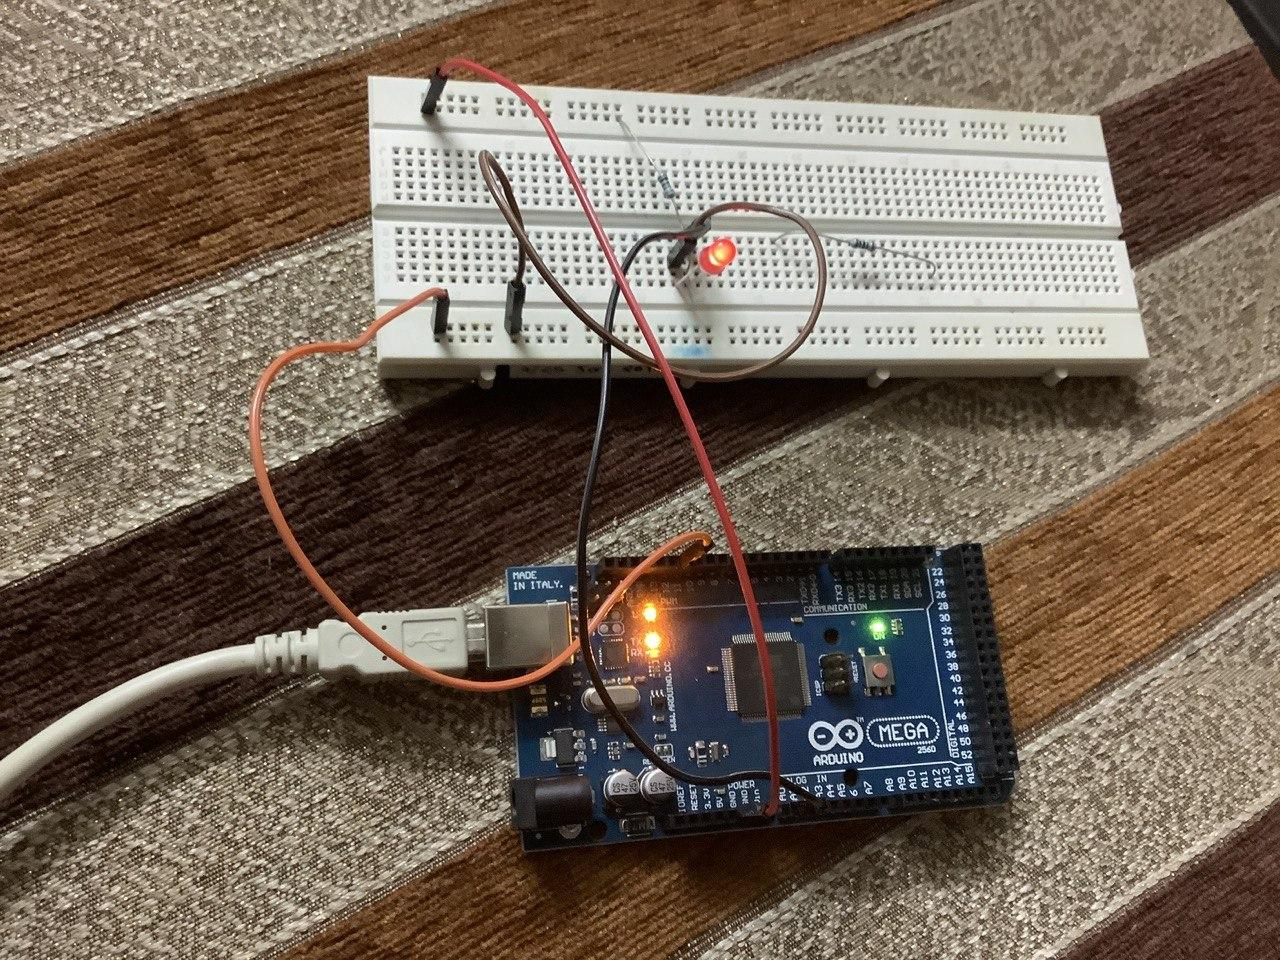
\includegraphics[width=\textwidth]{fig/pwm-high.jpg}
            \caption{Input \texttt{10}}
            \label{subfig:pwmlow}            
        \end{subfigure}
        \caption{Connected PWM Circuit.}
        \label{fig:pwmconnected}
    \end{figure}

    \begin{enumerate}
        \item The PWM setup works by adjusting the duty cycle of a digital output to
        obtain an apparent average analog voltage. This exploits the fact that due to
        persistence of vision, the light output of the LED connected to this voltage
        will also be averaged out, to appear dimmer over a period significantly longer
        than the PWM frequency. A slow-mo camera can easily catch this.
        \item The voltage is measured with the circuit in Figure \ref{subfig:pwmledcirc} with 
        the code in Figure \ref{subfig:pwmledcode}. A photo of the physical system has been 
        attached already in Figure \ref{fig:pwmconnected}. \\
        The output can be inaccurate due to current flowing, so this is mitigated by simply
        using enormous resistors in series. The output received consistently relayed 2.01V,
        close enough for a red LED (expected 1.8-2.1V).
    \end{enumerate}

    \begin{figure}[ht]
        \centering
        \begin{subfigure}[b]{0.3\textwidth}
            \scalebox{0.9}{\input{fig/ledpwm.pdf_tex}}
            \caption{Diagram of the circuit used.}
            \label{subfig:pwmledcirc}            
        \end{subfigure}
        \begin{subfigure}[b]{0.8\textwidth}
            \begin{lstlisting}[language=C++]
    void setup(){
        Serial.begin(115200);   // why not
        pinMode(11, OUTPUT);    // PWM pin
        pinMode(A0, INPUT);     // Voltage measuring pin
        analogWrite(11, 130);
    }

    void loop(){
        // convert to voltage and subtract from Vcc to get the drop
        Serial.println(5 - 5 * ((float)analogRead(A0) / (float) 1023));
    }
            \end{lstlisting}
            \caption{Code sent to the Arduino}
            \label{subfig:pwmledcode}            
        \end{subfigure}
        \caption{Measuring LED threshold voltage}
        \label{fig:pwmled}
    \end{figure}

    \questionpart
    We can store the output of the analog pin via an analog read (code in Appendix) and
    return it via serial after a set number of iterations. A possible other solution is 
    to return the current output via serial every time it is read, with a baud rate of say, 1M,
    not sure if that would give more resolution, but it would be less reliable due to cables and 
    USB interfaces being involved, not to mention, syncing serials of Arduino and the PC. 

    \begin{figure}[ht]
        \centering
        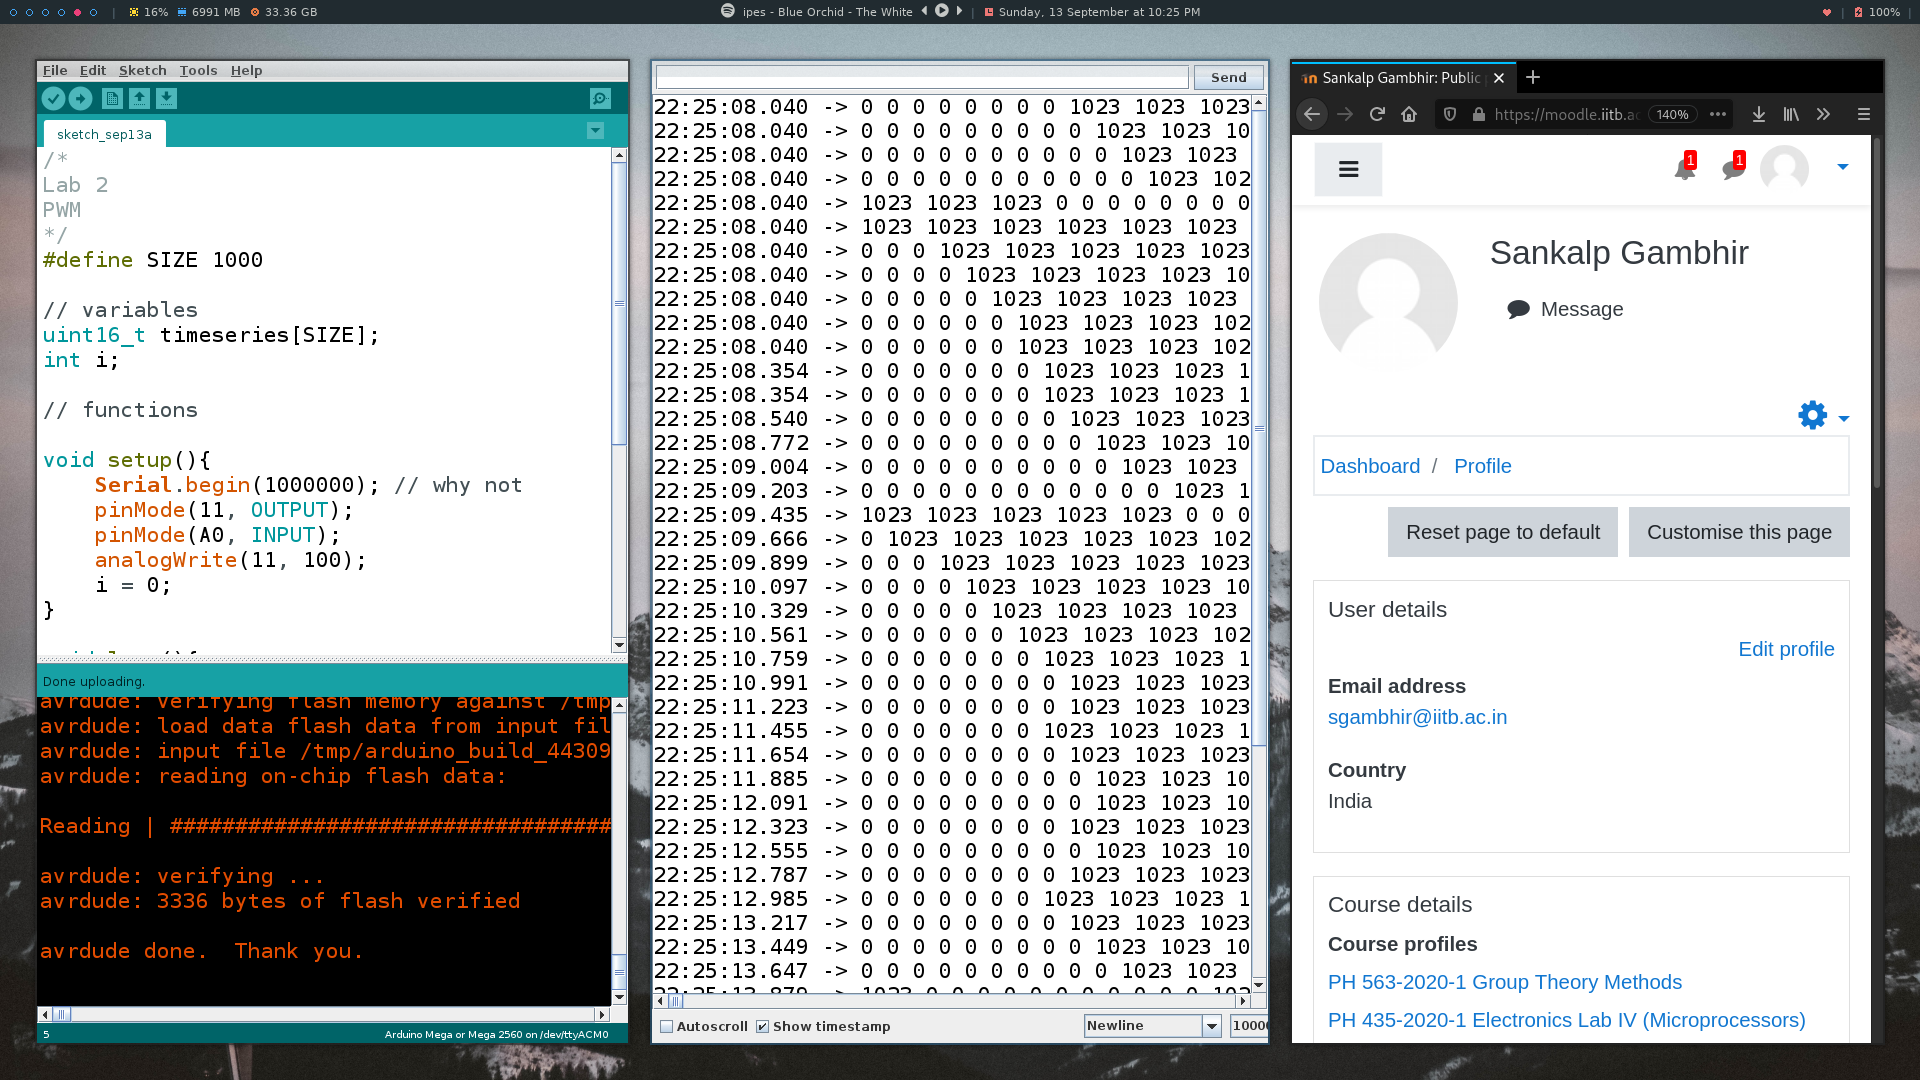
\includegraphics[width=0.8\textwidth]{fig/pwmproof.png}
    \end{figure}

    A rough calculation of the duty cycle can be done by counting the numbers of zeroes and 
    1023's obtained and taking their ratio. This was correct to within $3-4\%$ for values I tested,
    ranging between 50 and 200. The difference may be attributed to the frequency we have, getting
    around 20 readings for each cycle of the PWM wave.

    \questionpart
    The question was quite confusing about its intention, so I am assuming we had to 
    double the value of a DC analog signal after the PWM filtering.
    We can simply use a voltage pump to double the analog voltage. See Figure \ref{fig:voltmul}.
    The PWM wave itself can be easily used as a clock here.

    \begin{figure}[ht]
        \centering
        \scalebox{0.8}{\input{fig/voltdouble.pdf_tex}}
        \caption{Voltage doubler.}
        \label{fig:voltmul}        
    \end{figure}

    \begin{figure}[ht]
        \centering
        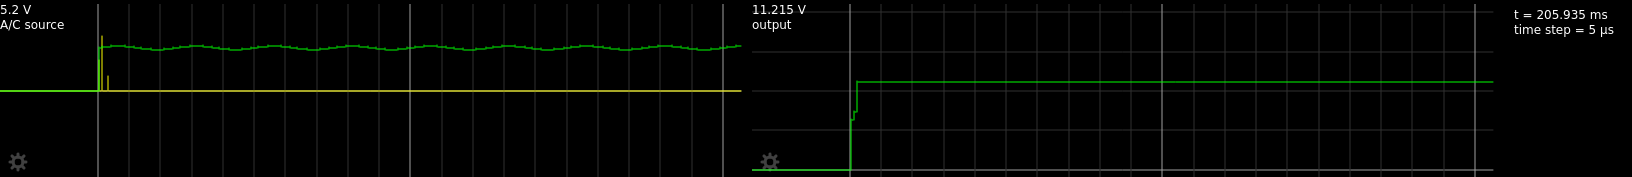
\includegraphics[width=0.9\textwidth]{fig/voldubsim.png}
        \caption{Voltage doubler simulation.}
        \label{fig:voltmulsim}                
    \end{figure}


\end{arabicparts}